\documentclass{article}
\usepackage[utf8]{inputenc}
\usepackage{graphicx}
\usepackage{epstopdf}
\usepackage{caption}
\usepackage{subcaption}
\usepackage{multirow}
\usepackage{hyperref}
\usepackage{url}
\usepackage{seqsplit}
\hypersetup{pdfstartview={FitH null null null}}
\usepackage{amssymb,amsmath}
\usepackage{amsthm}
\usepackage{empheq}
\usepackage{algorithm,algpseudocode}
\usepackage[margin=1.5in]{geometry}
\usepackage{listings}
\lstset{language=Python} 

\usepackage{listings}
\usepackage{color} %red, green, blue, yellow, cyan, magenta, black, white
\definecolor{mygreen}{RGB}{28,172,0} % color values Red, Green, Blue
\definecolor{mylilas}{RGB}{170,55,241}


\title{Ab-initio modeling using a fragment matching and energy functions}
\author{Caiwei Wang, Xiaokai Qian, Sean Lander, Haipei Fan, Puneet Gaddam, Brett Koonce\\University of Missouri - Columbia}

\date{March 10, 2013}

\algloopdefx{NoEndIf}[1]{\textbf{If} #1 \textbf{then}}

\begin{document}

\maketitle

\section{Abstract}
We model a CASP-10 template free target using ab initio modeling.  First, we construct a database of phi-psi angles from known PDB files.  Next, we build an initial model by selecting same/similar protein sequences from the database.  Then, we utilize simulated annealing and an external energy function (dDFIRE) to improve our model iteratively.  Ultimately, we visualize the formation of our new protein model, some statistics generated during our modeling process, and discuss further improvements.

\section{Introduction}


\subsection{Pipeline}
\begin{figure}[H]
\begin{center}
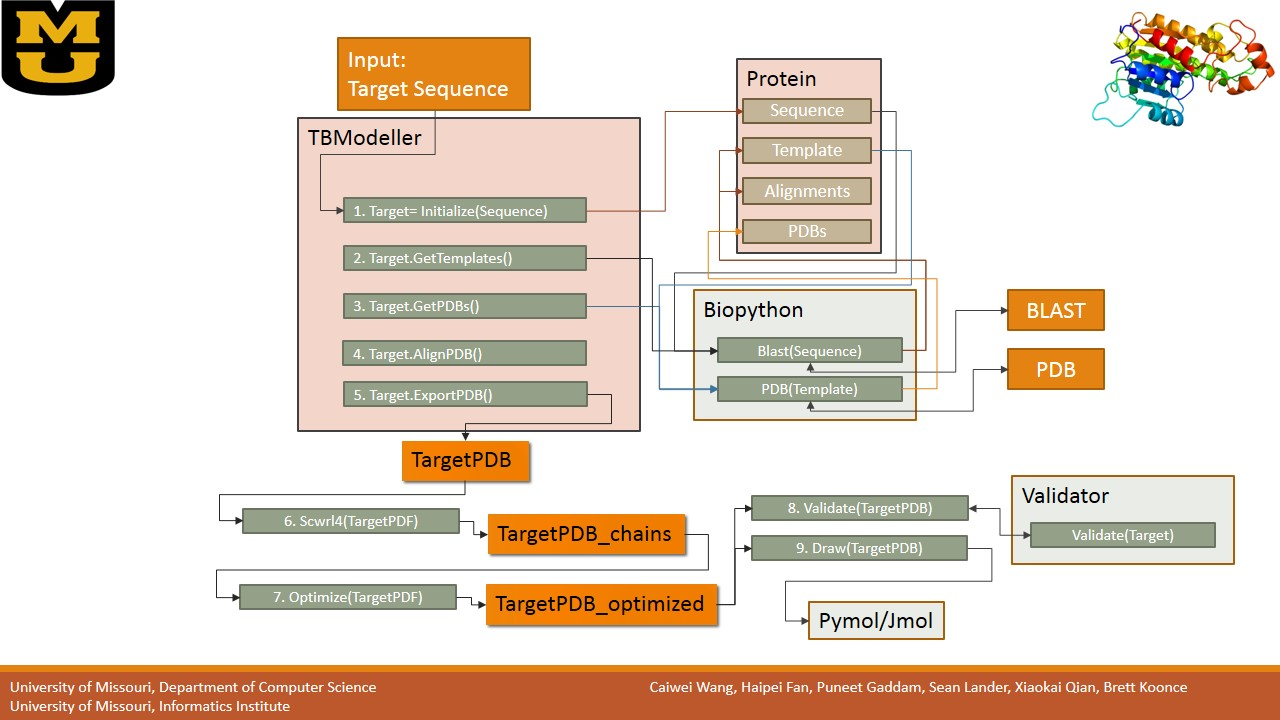
\includegraphics[width=\textwidth]{workflow}
\caption{An overview of the TBPy pipeline}
\label{Fig:blosum}
\end{center}
\end{figure}

\section{Target goal}

\subsection{CASP}

\section{Fragment database}

\section{Simulated annealing}

\subsection{d-DFIRE score}

\subsection{BLOSUM62 selection}


\section{Results/statistics}


\newpage
\section{Visualization}

After we obtain our final target PDB file, we use Jmol to visualize it. At the same time, we also visualize the native one to compare it with our prediction.  The left one is a target structure we generated (T0644), while right one is the native structure.

\begin{figure}
\centering
\begin{minipage}{.5\textwidth}
  \centering
  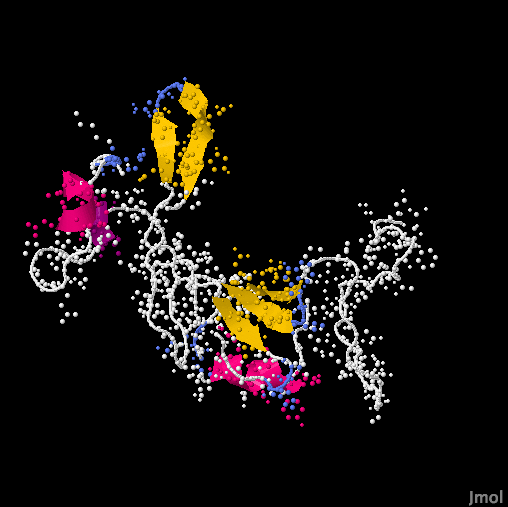
\includegraphics[width=.9\linewidth]{target_group_v2}
  \captionof{figure}{Target structure}
  \label{fig:test1}
\end{minipage}%
\begin{minipage}{.5\textwidth}
  \centering
  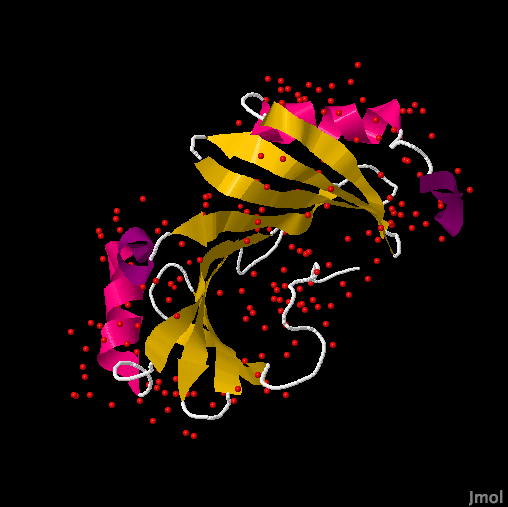
\includegraphics[width=.9\linewidth]{target_native}
  \captionof{figure}{Native structure}
  \label{fig:test2}
\end{minipage}
\end{figure}

\section{Results}



\subsection{Scores}
\begin{center}
    \begin{tabular}{ | l | l | l | p{2cm} |}
    \hline
      & Group1 & MULTICOM & MuFold \\ \hline
    TM-Score & 0.9971 & 0.9072 & 0.1985 \\ \hline
    RMSD & 0.23 & 1.666 & 14.978 \\
    \hline
    \end{tabular}
\end{center}

\section{Citations}

We thank the following tools and papers: \\\\




\end{document}


\end{document}
